\newsection
\subsection{Schnelle Fourier Transformation}
Da es viele Anwendungen für die Fourier-Transformation gibt, ist ein Algorithmus mit guter Laufzeit sehr wichtig.
Während eine naive version des DFT-Algorithmus eine Laufzeit von $\tco{N^2}$ hat,
so hat der Fast Fourier Transform Algorithmus nur eine Laufzeit von $\tco{N \log(N)}$,
was bei $N = 1024$ bereits eine Laufzeitsverbesserung von $100\times$ mit sich bringt ($\tco{10\,000}$ vs $\tco{1\,000\,000}$ Operationen)!
Die untenstehende Abbildung \ref{fig:trigo-interp-fft-runtimes} findet sich, zusammen mit dem Code,
mit der sie produziert wurde im Skript auf Seite 86-88

\begin{figure}[h!]
    \begin{center}
        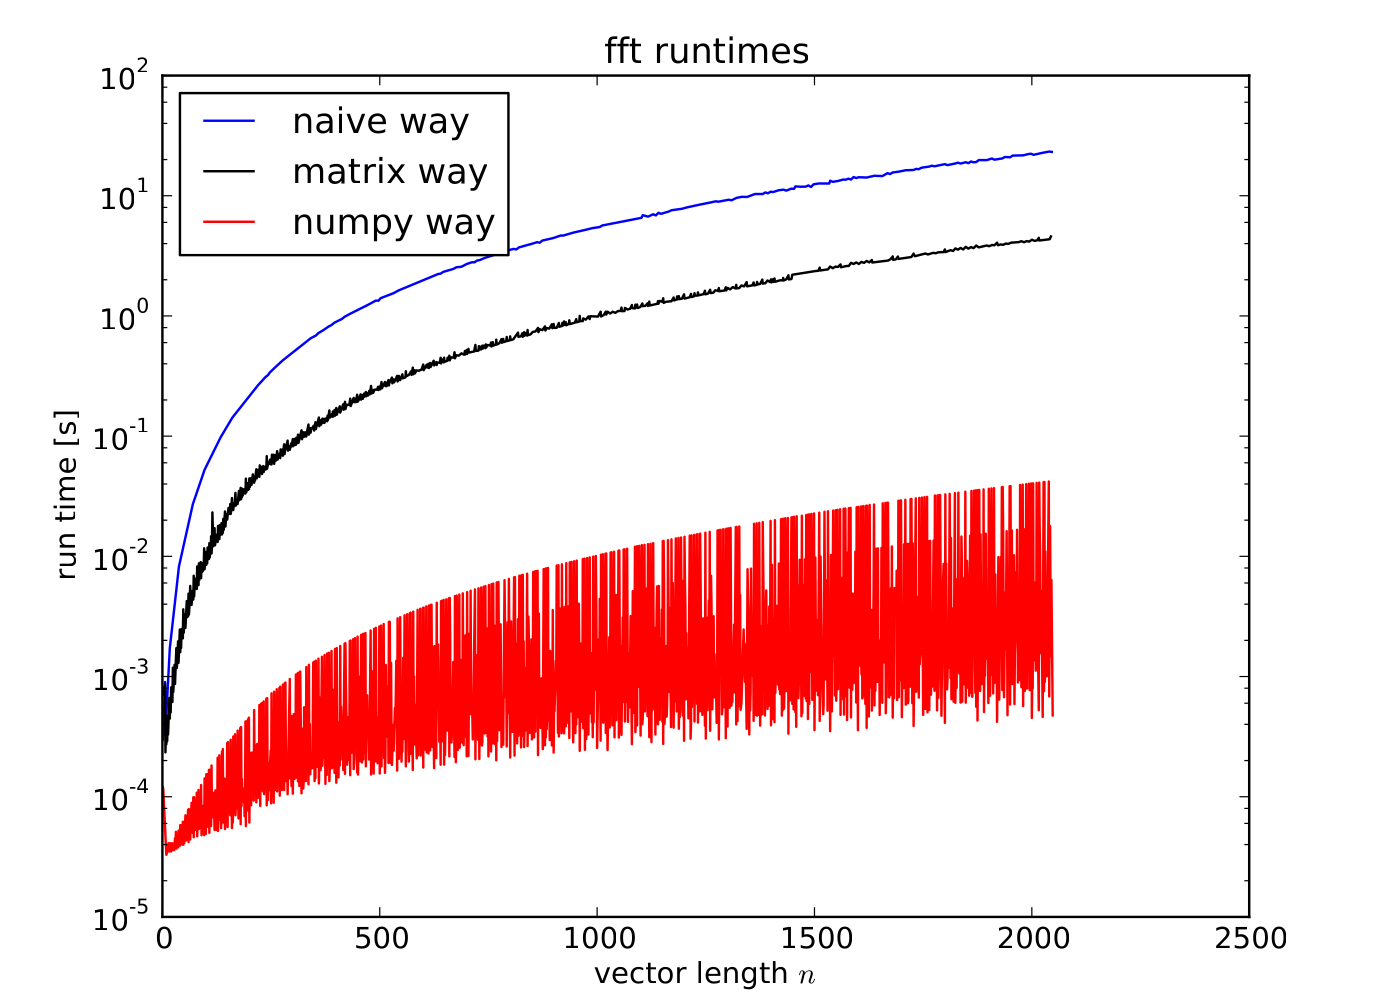
\includegraphics[width=0.7\textwidth]{assets/01_interpolation/01_trigonometric/fft-runtimes.png}
    \end{center}
    \caption{Vergleich der Laufzeit von verschiedenen Fourier-Transformations-Algorithmen}
    \label{fig:trigo-interp-fft-runtimes}
\end{figure}

Der hier besprochene Cooley-Tukey-Algorithmus wurde ursprünglich von Gauss 1805 entdeckt, dann vergessen und schliesslich 1965 von Cooley und Tukey wiederentdeckt.
Der Algorithmus verwendet einen ``Divide and Conquer'' Approach, also ist logischerweise die Idee,
dass man die Berechnung einer DFT der Länge $n$ auf die Berechnung vieler DFTs kleinerer Längen zurückführen kann.

Für den Algorithmus müssen folgende vier Optionen betrachtet werden:
\begin{enumerate}[label=\Roman*]
    \item Vektoren der Länge $N = 2m \Longrightarrow$ Laufzeit ideal
    \item Vektoren der Länge $N = 2^L \Longrightarrow$ Laufzeit ideal
    \item Vektoren der Länge $N = pq$ mit $p, q \in \Z \Longrightarrow$ Etwas langsamer
    \item Vektoren der Länge $N$, mit $N$ prim $\Longrightarrow$ ca. $\tco{N^2}$, besonders für $N$ gross
\end{enumerate}
Wir formen die Fourier-Transformation um für den ersten Fall ($N = 2m$):
\begin{align*}
    c_k & = \sum_{j = 0}^{N - 1} y_j e^{- \frac{2\pi i}{N} jk}                                                                     \\
        & = \sum_{j = 0}^{m - 1} y_{2j} e^{-\frac{2 \pi i}{N}2jk} + \sum_{j = 0}^{m - 1} y_{2j + 1} e^{-\frac{2\pi i}{N}(2j + 1)k} \\
        & = \sum_{j = 0}^{m - 1} \left( y_{2j} e^{-\frac{2 \pi i}{N \div 2}jk} \right)
    + e^{- \frac{2\pi}{N} k} \left( \sum_{j = 0}^{m - 1} y_{2j + 1} e^{-\frac{2\pi i}{N \div 2}jk} \right)
\end{align*}
Der zweite Fall ist einfach eine rekursive Weiterführung des ersten Falls,
bei welchem dann das $m$ kontinuierlich weiter dividiert wird bis zum Trivialfall mit einer $1 \times 1$-Matrix.

